\documentclass{llncs}
\usepackage{amsmath,amssymb,url}
\usepackage{algorithm}
\usepackage{algpseudocode}
\usepackage{graphicx}
\usepackage{mathcomp}

\newcommand{\Cyc}{\mathrm{\Phi}}
\newcommand{\Frob}{\mathrm{\Phi}}
\newcommand{\twist}{\mathrm{\Psi}}
\newcommand{\F}{\mathbb{F}}
\newcommand{\half}[1]{{\lfloor#1/2\rfloor}}
\newcommand{\ord}{\qopname\relax{no}{ord}}
\newcommand{\sign}{\qopname\relax{no}{sign}}
\newcommand{\tr}{\qopname\relax{no}{tr}}
\newcommand{\Z}{\mathbb{Z}}
\newcommand{\Cpp}{C\kern-0.05em\texttt{+\kern-0.03em+}}
\newcommand{\pp}{\,\kern-0.05em\texttt{+\kern-0.031em+}}
\newcommand\T{\rule{0pt}{2.6ex}}

\newcommand{\Input}{\item[\textsc{Input:}]}
\newcommand{\Output}{\item[\textsc{Output:}]}

\sloppy

\begin{document}

\pagestyle{plain}

\title{The Apache Milagro Crypto Library (Version 2.0)}

\author{
Michael Scott 
}

\institute{}

\institute{
%Chief Cryptographer \\
MIRACL Labs\\%
%\bf{For Internal Distribution Only} \\
\email{mike.scott@miracl.com} \\
}

\maketitle

\begin{abstract}

We introduce a new multi-lingual crypto library, specifically designed to support the Internet of Things.

\end{abstract} 

\section{Introduction}\label{sec:intro}

%One of the major mysteries in the real-world of crypto is resistance to the exploitation of new research ideas. Its not that cryptographic research has failed to throw up new ideas that have
%the potential for commercial exploitation -- far from it. But in the real-world 1970's crypto rules supreme, and very little happens that isn't PKI/RSA based. The reasons for this are many and varied.
%However one part of the puzzle might be the non-availability of easy-to-use open source cryptographic tools, that do not require in depth cryptographic expertise to deploy.

%In particular 
There are many crypto libraries out there. Many offer a bewildering variety of cryptographic primitives, at different levels of security. Many use extensive assembly language 
in order to be as fast as possible. Many are very big, even bloated. Some rely on other external libraries. Many were designed by academics for academics, and so are not really suitable for 
commercial use. Many are otherwise excellent, but not written in our favourite language.

The Apache Milagro Crypto Library (AMCL) \footnote{\url{https://github.com/MIRACL/amcl.git}} is different. AMCL is completely self-contained (except for the requirement for an external entropy source for random number generation). 
AMCL is for use in the pre-quantum era -- that is in the here and now. With 
the advent of a workable quantum computer, AMCL will become history. But we are not expecting that to happen any time soon.

AMCL is portable -- there is no assembly language. The original version is written in C, Java, Javascript, Go and Swift using only generic programming constructs, but AMCL is truly 
multi-lingual, as compatible 
versions will be available in many other languages (see below). These versions will be identical in that for the same inputs they will not only produce the same outputs, but all internal calculations will also be the same. 
AMCL is fast, but does not attempt to set speed records (a particular academic obsession). There are of course contexts where speed is of the essence -- for example for a server farm which must handle 
multiple SSL connections, and where a 10\% speed increase implies the need for 10\% less servers, with a a 10\% saving on electricity. But in the Internet of Things we would suggest that this is less 
important. In general the speed
is expected to be ``good enough''. However AMCL is small. Some libraries boast of having hundreds of thousands of lines of code - AMCL has less than 10,000. AMCL takes up the minimum of 
ROM/RAM resources in order to fit into the smallest possible embedded footprint, consistent with other design constraints. It is expected that this will be vital for implementations that 
support security in the Internet of Things. AMCL (the C version) only uses stack memory, and is thus natively multi-threaded.

The original version of AMCL supported only one level of security, equivalent to 128-bit AES. Rather relunctantly we have removed this constraint and this version supports all levels of security up to
the 256-bit AES level. This was motivated by the observation that there will always be a demand for higher levels of crypto-security, even if such measures are unlikely to improve a systems overall security. 

AMCL makes most 
of the choices for you as to which primitives to use, based on the best available current advice. Specifically it uses AES/128/192/256 for symmetric encryption, SHA256/384/512 for hashing, prime field elliptic
curves for public key protocols, and BN and BLS curves to support pairing-based protocols. However three different parameterizations of Elliptic curve are supported - Weierstrass, Edwards and 
Montgomery, as each is appropriate within its own niche. In each case only the standard projective coordinates are used. But you do get to 
choose the actual elliptic curve, with support for three different 
forms of the modulus. For pairings we assume a modulus congruent to $3 \bmod 8$ with a D-type twist \cite{barreto-naehrig}, \cite{barreto-lynn-scott}.
Standard modes of AES are supported, plus GCM mode for authenticated encryption.

The C version of AMCL is configured at compile time for 16, 32 or 64 bit processors, and for a specific elliptic curve. The Java and Javascript versions are (obviously) processor agnostic, 
but the same choices of elliptic curve are available.

AMCL is written with an awareness of the abilities of modern pipelined processors. In particular there was an awareness that the unpredictable program branch should be avoided, not 
only as it slows down the processor, but as it may open the door to side-channel attacks. The innocuous looking {\tt if} statement -- unless its outcome can be accurately predicted -- is the enemy 
of quality crypto software.

In the sequel we refer to the C version of AMCL, unless otherwise specified. We emphasis that all AMCL versions are completely self-contained. No external 
libraries or packages are required to implement all of the supported cryptographic functionality (other than for an external entropy source). However we do recognise the need to
support X509 standards, which while requiring no cryptographic code per se, are often required to interface closely with it. Most languages provide their own X509 packages, so we will not
attempt to replicate that functionality here. However the C version of AMCL does include a basic X509 module.

\section{Context}

A crypto library does not function is isolation. The AMCL was originally designed to support the MIRACL IoT solution. The MIRACL IoT solution is based on a cloud-based infrastructure designed by MIRACL 
to support the M-Pin protocol \cite{mpin}, but which has wider application to novel protocols of particular relevance to the IoT. This document describes the AMCL library which was originally designed for internal use, 
but which has now reached a level of maturity where we are pleased to make it available as a service to the wider community as an open source product, under a standard Apache 2.0 license.

\section{Library Structure}

The modules that make up AMCL are shown below, with some indication of how they interact. Several example APIs will be provided to implement common protocols. Note that all
interaction with the API is via machine-independent endian-indifferent arrays of bytes (a.k.a. octet strings). 
Therefore the underlying workings of the library are invisible to the consumer of its services.

\begin{figure}[!htb]
  \begin{center}
    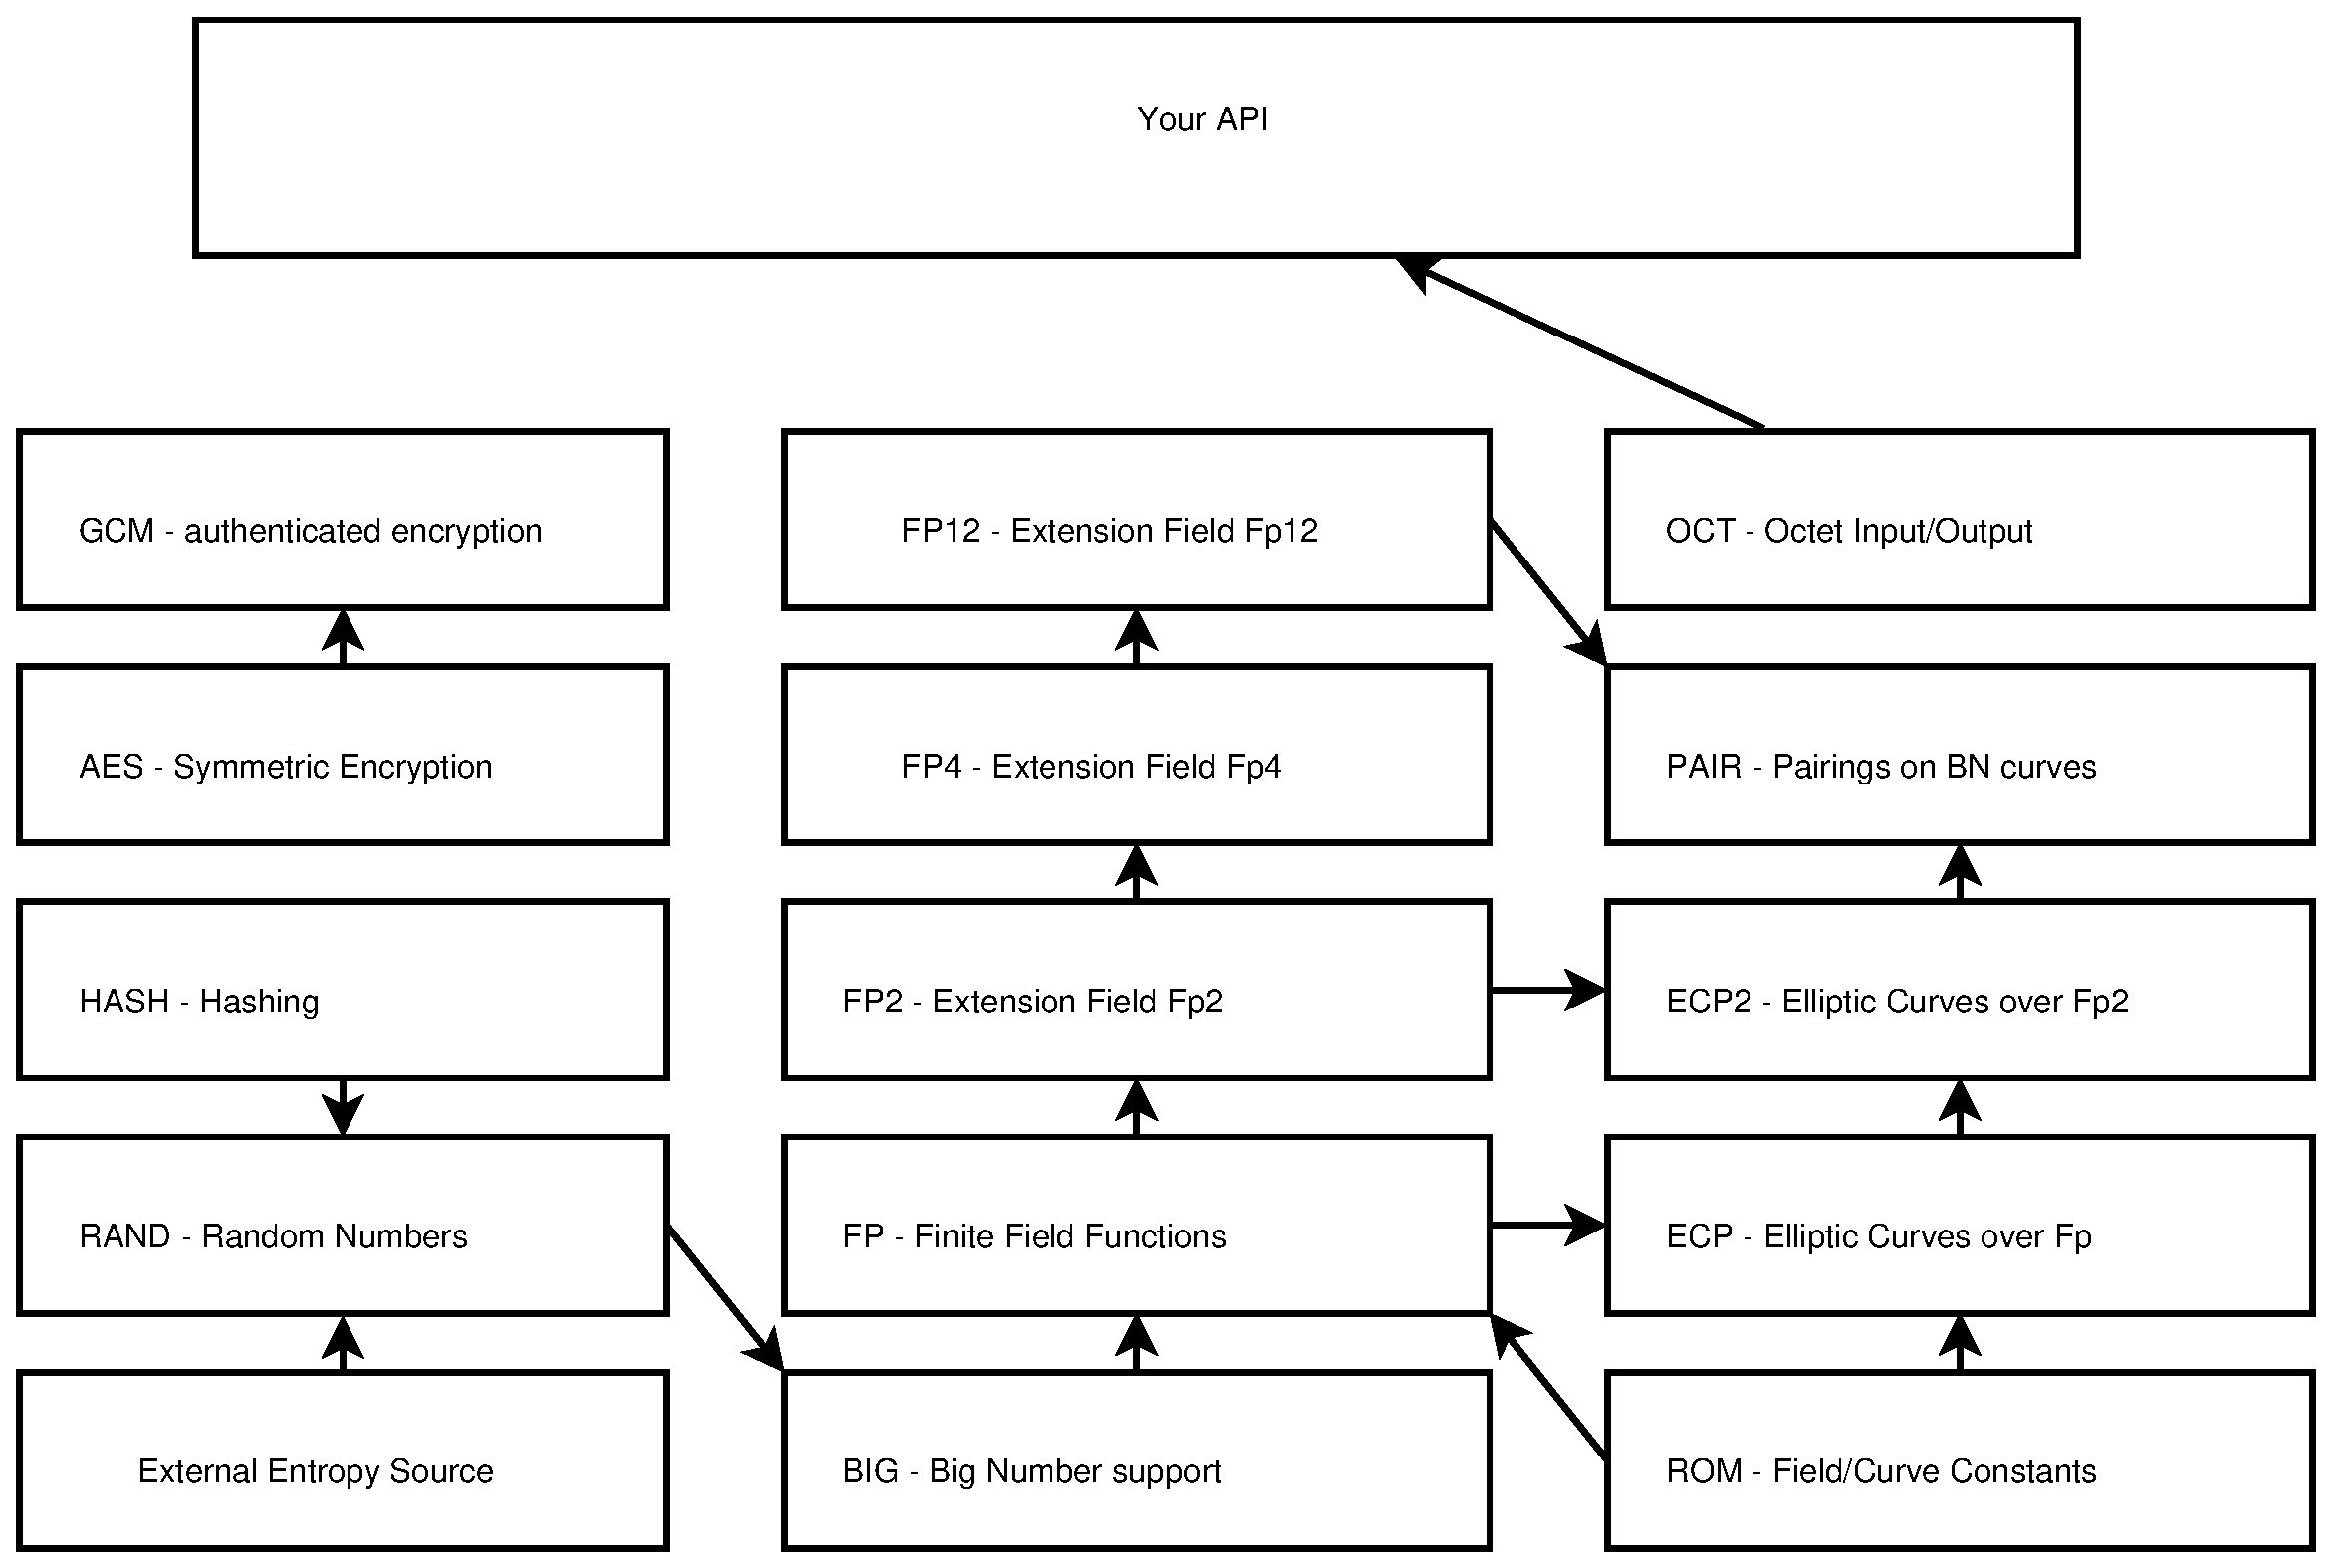
\includegraphics[width=120mm ]{clint.eps}
  \end{center}
  \caption{\small The AMCL library.}
  \label{clint}
\end{figure}

The symmetric encryption and hashing code, along with the random number generation, is uninteresting, and since we make no claims for it, we will not refer to it again. It was mostly
borrowed from our well-known MIRACL library.

\section{Handling Big Numbers}

\subsection{Representation}

One of the major design decisions is how to represent the field elements required for the elliptic curve and pairing-based cryptography. 
Clearly some multi-precision representation will be required.  Here there are two different approaches. 
One is to pack the bits as tightly as possible into computer words. For example on a 64-bit computer 256-bit numbers can be stored in just 4 words. However to manipulate numbers in this 
form, even for simple addition, requires handling of carry bits if overflow is to be avoided, 
and a high-level language does not have direct access to carry flags. It is possible to emulate the flags, but this would be inefficient. In fact this approach is only really suitable 
for an assembly language implementation.

The alternative idea is to use extra words for the representation, and then try to offset the additional cost by taking full advantage of the ``spare'' bits in every word. 
This idea follows a ``corner of the literature'' \cite{bernstein-chuengsatiansup-lange} which has been promoted by Bernstein and his collaborators in several publications.
Refer to figure \ref{words}, where each digit of the representation is stored as a signed integer which is the size of the processor word-length. Recently it has been 
demonstrated that such a reduced-radix representation can take advantage of a simple form of Karatsuba multiplication to significantly reduce its cost \cite{scott2}. 

Almost all arithmetic takes place modulo a prime number, the modulus representing the field over which the elliptic curve is defined, here denoted as $p$.
Care must be taken to ensure that the choice of number base allows for numerical stability -- in practice integer arithmetic overflow must never occur. Normally the maximum
number base possible should be used. A small utility is provided with the library to assist with this choice. For example for a 32-bit processor a base of $2^{29}$ is almost
always optimal.

As well as a ``word excess'' (that is the number of unused bits in every digit, excluding the sign bit), there should also be a ``field excess'', that is a number of extra spare bits in the most 
significant digit of the representation. This faciliates so-called lazy reduction (see below).

For example for a 256-bit prime modulus on a 32-bit computer, representing field elements to the base $2^{29}$ allows a word excess of 2 bits and a field excess of 5 bits. The overall
representation consists of 9 digits.

Such a representation of a big number is referred to as a {BIG}. Addition or subtraction of a pair of {BIG}s, results in another {BIG}.

The Java version uses exactly the same 32-bit representation as above. For Javascript (where all numbers are stored as 64-bit floating point with a 52-bit mantissa, but mostly 
manipulated as 32-bit integers), an effective word length of 26 bits is assumed.

\subsection{Addition and Subtraction}

The existance of a word excess means for example that multiple field elements can be added together digit by digit, without processing of carries, before overflow can occur. 
Only occasionally will there be a requirement to {\it normalise} these {\it extended} values,  that is to force them back into the original format. Note that this is independent of the modulus.

The existance of a field excess means that, independent of the word excess, multiple field elements can be added together before it is required to reduce the sum with respect to the modulus. In the 
literature this is referred to as lazy, or delayed, reduction.

Note that these two mechanisms associated with the word excess and the field excess (often confused in the literature) operate largely independently of each other.

AMCL has no support for negative numbers. Therefore subtraction will be implemented as field negation followed by addition. Negation is performed using the method described as 
Option 1 in \cite{aranha-karabina-longa-gebotys-lopez}. Basically the 
number of the active bits in the field excess of the number to be negated is determined, the modulus is shifted left by this amount plus one, and the value to be negated is subtracted from this value.
Note that because of the ``plus 1'', this will always produce a positive result at the cost of eating a bit into the field excess.

\begin{figure}[!htb]
  \begin{center}
    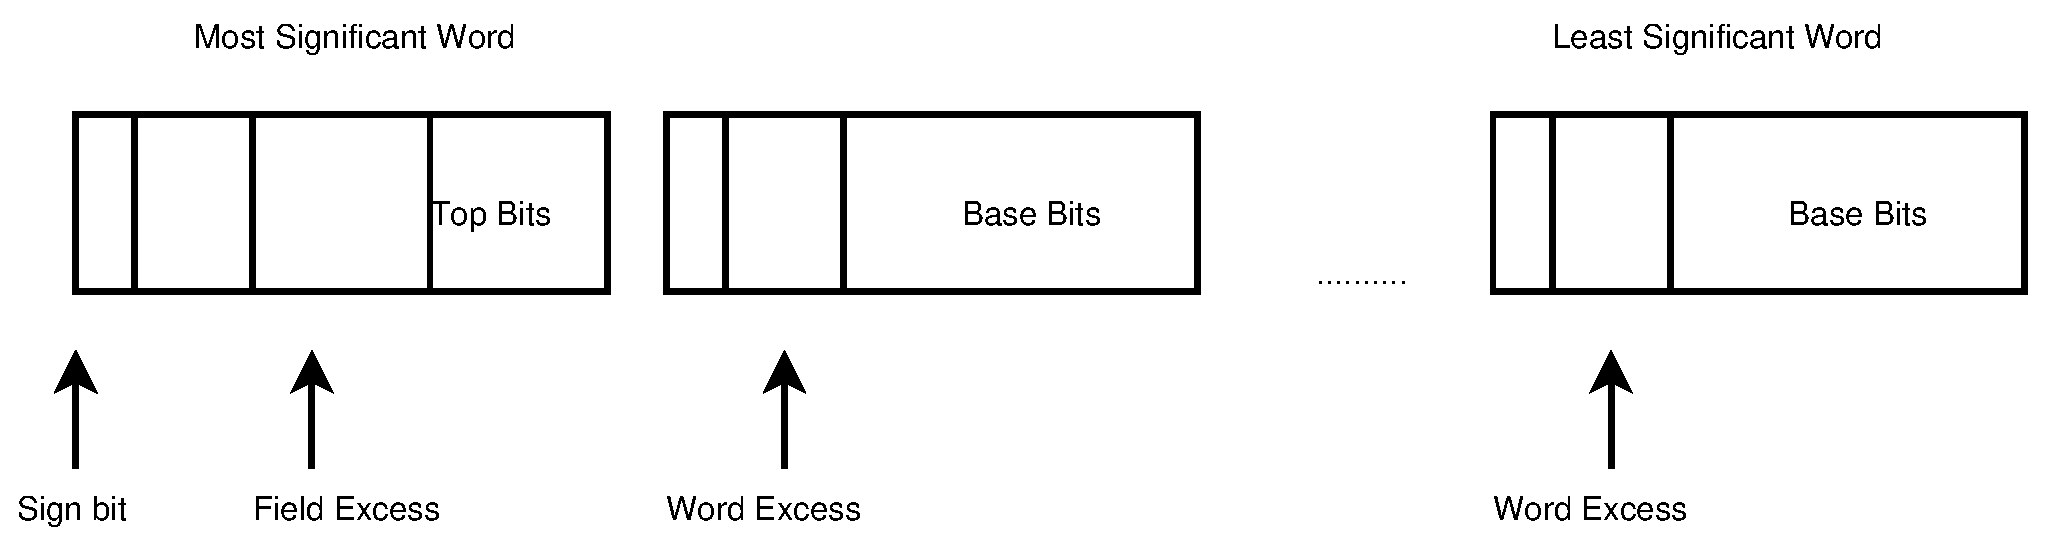
\includegraphics[width=120mm ]{words.eps}
  \end{center}
  \caption{\small Big number representation}
  \label{words}
\end{figure}

Normalisation of extended numbers requires the word excess of each digit to be shifted right by the number of base bits, and added to the next digit, working right to left. Note that when numbers 
are subtracted digit-by-digit individual digits may become negative. However
since we are avoiding using the sign bit, due to the magic of 2's complement arithmetic, this all works fine without any conditional branches.

Reduction of unreduced {BIG} numbers is carried out using a simple shift-compare-and-subtract of the modulus, with one subtraction needed on average half of the time for every active bit in the field excess. 
Hopefully such reductions will rarely be required, as they are slow and involve unpredictable program branches.

Since the length of field elements is fixed at compile time, it is expected that the compiler will unroll most of the time-critical loops. In any case the conditional branch required at the foot of a 
fixed-size loop can be accurately predicted by modern hardware.

The problem now is to decide when to normalise and when to reduce numbers to avoid the possibility of overflow. There are two ways of doing this. One is to monitor the excesses at run-time and act when the 
threat of overflow arises. The second is to do a careful analysis of the code and insert normalisation and reduction code at points where the possibility of overflow may arise, based on a static worst-case 
analysis. 

The field excess $E_n$ of a number $n$ is easily captured by a simple masking and shifting of the top word. If two normalised numbers $a$ and $b$ are to be added then the excess of their sum will be at worst 
$E_a + E_b +1$. As long as this is less than $2^{FE}$ where $FE$ is the field excess, then we are fine. Otherwise both numbers should be reduced prior to the addition. In AMCL these checks are 
performed at run-time. However, as we shall see, in practise these reductions are very rarely required. So the {\tt if} statement used to control them is highly predictable. Observe that even
in the worst case, for a 16-bit implementation, the excess is a generous $FE=4$, and so many elements can be added or subtracted before reduction is required.

The worst case word excess for the result of a calculation is harder to calculate at run time, as it would require inspection of every digit of every {BIG}. This would slow computation down to an unacceptable extent. 
Therefore in this case
we use static analysis and insert normalisation code where we know it might be needed. This process was supported by special debugging code that warned of places where overflow was possible, based on a simple
worst-case analysis.

\subsection{Multiplication and Reduction}

To support multiplication of {BIG}s, we will require a double-length {DBIG} type. Also the partial products that arise in the process of long multiplication will require a double-length data type. Fortunately many 
popular C compilers, like Gnu {GCC}, always support an integer type that is double the native word-length. For Java the ``int'' type is 32-bits and there is a double-length ``long'' type which is 64-bit.
Of course for Javascript a double length type is not possible, and so the partial products must be accomodated within the 52-bit mantissa.

Multiprecision multiplication is performed column by column, propagating the carries, working from right-to-left, but using the fast method described in \cite{scott2}.
At the foot of each column the total is split into the sum for that column, and the carry to the next column. If the numbers are normalised 
prior to the multiplication, then 
with the word excesses that we have chosen, this will not result in overflow. The {DBIG} product will be automatically normalised as a result of this process. Squaring can be done in a 
similar fashion but at a slightly lower cost. 

The {DBIG} value that results from a multiplication or squaring may be immediately reduced with respect to the modulus to bring it back to a {BIG}. However again we may choose to delay this 
reduction, and therefore we need the ability to safely add and subtract DBIG numbers while again avoiding overflow.

The method used for full reduction of a DBIG back to a BIG depends on the form of the modulus. We choose to support three distinct types of modulus, (a) pseudo Mersenne of the form $2^n-c$ where 
$c$ is small and $n$ is the size of the modulus in bits, 
(b) Montgomery-friendly of the form $k.2^n-1$, and (c) moduli of no special form. For cases (b) and (c) we convert all 
field elements to Montgomery's {\it n}-residue form, and use Montgomery's fast method for modular reduction \cite{montgomery}, \cite{scott2}. In all cases the DBIG number to be reduced $y$ must be in the 
range $0<y<pR$ (a requirement of Montgomery's method), and the result $x$ is guaranteed to 
be in the range $0<x<2p$, where $R=2^{M+FE}$ for an M-bit modulus. Note that the BIG result will be (nearly) fully reduced. The fact than we allow $x$ to be larger than $p$ means that we can avoid
the notorious Montgomery ``final subtraction'' \cite{montgomery}.

Observe how unreduced numbers involved in complex calculations tend to be (nearly fully) reduced if they are involved in a modular multiplication. So for example if field element $x$ has a large field excess,
and if we calculate $x=x.y$, then as long as the unreduced product is less than $pR$, the result will be a nearly fully reduced $x$. So in many cases there is a natural tendency for field excesses 
not to grow without limit, and not to overflow, without requiring explicit action on our part.

Consider now a sequence of code that adds, subtracts and multiplies field elements, as might arise in elliptic curve additions and doublings. Assume that the code has been analysed and that normalisation 
code has been inserted where needed. Assume that the reduction code that 
activates if there is a possibility of an element overflowing its field excess, while present, never in fact is triggered (due to the behaviour described above). Then we assert that there is only one 
possible place in which an unpredicted branch may occur. This will be in the negation code associated with a subtraction, where the number of bits in the field excess must be counted. However we would 
point out that some architectures do now support machine code instructions that count the number of active bits in a computer register -- although unfortunately this capability is not supported by the 
typical high-level language syntax.

\section{Extension Field arithmetic}

To support cryptographic pairings we will need support for extension fields. We use a towering of extensions, from $\F_p$ to $\F_{p^2}$ to $\F_{p^4}$ to $\F_{p^{12}}$ as required for 
BN \cite{barreto-naehrig} and BLS \cite{barreto-lynn-scott} curves. An element 
of the quadratic extension field will be represented as $f=a+ib$, where $i$ is the square root of the quadratic non-residue -1.
To add, subtract and multiply them we use the obvious methods. However for negation we can construct $-f=-a-ib$ as $b-(a+b)+i.(a-(a+b)$ which requires only one base field negation. A similar idea 
can be used recursively for higher order extensions, so that only one base field negation is ever required.


\section{Elliptic Curves}

Three types of Elliptic curve are supported for the implementation of Elliptic Curve Cryptography (ECC), but curves are limited to popular families that support faster implementation. Weierstrass 
curves are supported using the Short Weierstrass representation:-

$$ y^2=x^3+Ax+B $$

where $A=0$ or $A=-3$. Edwards curves are supported using both regular and twisted Edwards format:-

$$ Ax^2+y^2=1+Bx^2y^2 $$

where $A=1$ or $A=-1$. Montgomery curves are represented as:-

$$ y^2=x^3+Ax^2+x $$

where $A$ must be small.

In the particular case of elliptic curve point multiplication, there are potentially a myriad of very dangerous side-channel attacks that arise from using the classic double-and-add algorithm
and its variants. Vulnerabilities arise if branches are taken that depend on secret bits, or if data is even accessed using secret values as indices.
Many types of counter-measures have been suggested. The simplest solution is to use a constant-time algorithm like the Montgomery ladder, which has a very simple structure, uses very little 
memory and has no key-bit-dependent branches. 
If using a Montgomery representation of the elliptic curve the Montgomery ladder \cite{montgomery2} is in fact the optimal algorithm for point multiplication. For other representations we use a 
fixed-sized signed window method, as described in \cite{bos-costello-longa-naehrig}. 

AMCL has built-in support for most standardised elliptic curves, along with many curves that have been proposed for standardisation. 
Specifically it supports the NIST256 curve \cite{certicom}, \cite{nist}, the well known Curve25519 \cite{bernstein}, the 256-bit Brainpool curve \cite{brainpool}, the ANSSI curve \cite{ANSSI}, and four
NUMS (Nothing-Up-My-Sleeve) curves proposed by Bos et al. \cite{bos-costello-longa-naehrig}. At higher levels of security the NIST384 and NIST521 curves are supported, also 
Curve41417 \cite{bernstein-chuengsatiansup-lange} as well as the Goldilocks curve \cite{hamburg}, and our own
Hi{F}ive curve \cite{scott3}.

Some of these proposals support only a Weierstrass representation, but many also allow an Edwards and Montgomery 
form. Tools are provided to allow easy integration of more curves.


\section{Support for classic Finite Field Methods}

Before Elliptic Curves, cryptography depended on methods based on simple finite fields. The most famous of these would be the well known RSA method. These methods have the advantage of
being effectively parameterless, and therefore the issue of trust in parameters that arises for elliptic curves, is not an issue. However these methods are subject to index calculus based
methods of cryptanalysis, and so fields and keys are typically much larger. So how to support a 2048-bit implementation of RSA based on a library designed for optimized operations on much smaller numbers? 
The idea is simple --
use AMCL as a virtual M-bit machine, where M is the bit length of the supported elliptic curve, and build RSA arithmetic on top of that. And to claw back some decent performance use the Karatsuba 
method \cite{knuth} so that for example 2048-bit multiplication
recurses efficiently right down to 256-bit operations. Of course the downside of the Karatsuba method is that while it saves on multiplications, the number of additions and subtractions is greatly increased.
However the existance of generous word excesses in our representation makes this less of a problem, as most additions can be carried out without normalisation. 

Secret key operations like RSA decryption use the Montgomery ladder to achieve side-channel-attack resistance.

The implementation can currently support $M.2^n$ bit fields. For example choosing $M=256$, 2048-bit RSA can be used to get reasonably close to the AES-128-bit level of security, and if desired 4096 bit RSA can be used to
comfortably exceed it. 

Note that this code is supported independently of the elliptic curve code. So for example $M.2^n$-bit RSA and $M$-bit ECC can be run together within a single application. 

However we regard these methods as ``legacy'' as in our view ECC based methods are a much better fit for the IoT. 

\section{Multi-Lingual support}

It is a big ask to develop and maintain multiple versions of a crypto library written in radically different languages such as C, Java, Javascript, Go and Swift. This has discouraged the use of
language specific methods (which are in any case of little relevance here), and strongly encouraged the use of simple, generic computer language constructs. 

This approach brings a surprising bonus: AMCL can be automatically converted to many other languages using available translator tools. For example Tangible Software Solutions \cite{tss}
market a Java to C\# converter. This generated an efficient fully functional C\# version of AMCL within minutes. The same company market a Java to Visual Basic converter. 
Google have a Java to Objective C
converter \cite{gol} specifically designed to convert Android apps developed in Java, to iOS apps written in Objective C.

Of course not all languages can be supported in this way, so support for some will be developed manually. In particular a Rust version is currently under development.


\section{Discussion}

We found in our code that, with few exceptions, reductions due to possible overflow of the field excess of a BIG were very rare, especially for the 64-bit version of the library. Similarly 
normalisation was 
rarely needed for the 64-bit code. This is due to the much greater excesses that can apply in the 64-bit representation. In some experiments we calculated thousands of random pairings, 
and reduction due to field excess overflow detection never happened.

In general in developing AMCL we tried to use optimal methods, without going to what we (very subjectively) regarded as extremes in order to maximise performance. 
Algorithms that require less memory were generally preferred if the impact on performance was not large. Some optimizations, while perfectly valid, are hard to 
implement without having a significant impact on program readability and maintainability. Deciding which optimizations to use and which to reject (on the grounds of code size and negative impact on code 
readability and maintainability) is admittedly rather arbitrary!

One notable omission from AMCL is the use of precomputation on fixed parameters in order to speed up certain calculations. We try to justify this, rather unconvincingly, by pointing out 
that precomputation must of necessity increase code size. Furthermore such methods are more sensitive to side-channel attacks and much of their speed advantage will be lost if they are to be 
fully side-channel protected. Also precomputation on secret values clearly increases the amount of secret data that needs to be protected.
However our view might change in later versions depending on our in-the-field experiences of using AMCL.

%\newpage
\bibliographystyle{plain}
\bibliography{amcl}

%\newpage
\appendix

\section*{Benchmarks}

Since AMCL is intended for the Internet of Things, we think it appropriate to give some timings based on an implementation on the Raspberry Pi (version 2) computer, which is
based on a 32-bit ARM7 chip. We do not overclock the 900MHz processor. 

We developed three API programs, one which tests standard methods of elliptic curve key exchange, public key cryptography and digital signature. Another implements all components of our M-Pin protocol,
a pairing-based protocol of medium complexity \cite{mpin}.  The former uses the ed25519 Edwards curve \cite{bernstein-duif-lange-schwabe-yang} with its pseudo-mersenne modulus, and the latter a 256-bit BN curve.
Finally we implement all the steps of the RSA public key encryption protocol using 2048-bit keys, that is key generation, encryption and decryption.

These might be regarded as representative of what might be expected for an implementation of a typical elliptic curve (ECC) protocol, a typical pairing-based (PBC) protocol, and a typical classic 
public key protocol based on RSA.
The results in the first table indicate the code and stack requirements when these programs were compiled using version 4.8 of the GCC compiler, using the standard  -O3 (optimize for best performance) and -Os
(optimize for minimum size) flags, and a flag to indicate the specific ARM architecture (Cortex-A7).


\begin{table}
\centering
\begin{tabular}{|l|c|c|}
\hline
&~~Code Size~~&~Maximum Stack Usage~\\
\hline
~ECC  -O3 & 68085 & 4140  \\  %
~ECC  -Os & 31115 & 3752 \\   %
~PBC  -O3 & 84031 & 8140 \\   %
~PBC  -Os & 46044 & 7904 \\   %
~RSA  -O3 & 61461 & 5332 \\   %
~RSA  -Os & 23449 & 5228 \\   %
\hline
\end{tabular}
~\\
\caption{Typical Memory Footprint}
\label{footprint}
\end{table}


Next we give some timings for a single SPA-protected ECC point multiplication on an Edwards curve, for the calculation of a single PBC pairing on the 256-bit BN curve, and for a SPA-protected 2048-bit RSA decryption.

\begin{table}
\centering
\begin{tabular}{|l|c|}
\hline
&~Time in milliseconds~\\
\hline
~ECC point multiplication -O3 & 3.9  \\ % 
~ECC point multiplication -Os & 5.9 \\ % 
~PBC pairing -O3 & 47.4 \\ % 
~PBC pairing -Os & 77.3 \\ % 
~RSA decryption -O3 & 155 \\  %  
~RSA decryption -Os & 233 \\  % 
\hline
\end{tabular}
~\\
\caption{C Benchmarks}
\label{cspeed}
\end{table}

Observe that we do not compare these timings with any other -- because that is not the point.
The point is -- are they ``good enough'' for whatever application you have in mind? And we suspect that, in the great majority of cases, they are.

Clearly for Java and Javascript we are completely at the mercy of the efficiency (or otherwise) of the virtual machine. As can be seen from these Javascript timings, these
can vary significantly.


\begin{table}
\centering
\begin{tabular}{|l|l|l|c|}
\hline
 & ~Device~ & ~Browser~ &~Time in seconds~\\
\hline
~ECC point multiplication~  & ~Raspberry Pi~ & ~Epiphany~ & 0.65  \\
  & ~Apple iPad 2~ & ~Safari~ & 0.096  \\
  & ~Samsung Galaxy Note 4~ & ~Chrome~ & 0.018  \\
~PBC pairing~  &  ~Raspberry Pi~ & ~Epiphany~ & 11.0\\
 &  ~Apple iPad 2~ & ~Safari~ & 1.6\\
 &  ~Samsung Galaxy Note 4~ & ~Chrome~ & 0.30\\
\hline
\end{tabular}
~\\
\caption{JavaScript Benchmarks}
\label{jsspeed}
\end{table}


\end{document}
